\documentclass[12pt]{article}
\usepackage{fullpage,graphicx,psfrag,amsmath,amsfonts,verbatim}
\usepackage[small,bf]{caption}
\usepackage{array}
\usepackage{multirow}
\usepackage{rotating}
\usepackage{relsize}
\usepackage{subcaption}

\input defs.tex

\bibliographystyle{alpha}

\title{ELE120: Assignment 1 \\ [0.1em]\smaller{}Representative report}
\author{Your name \textit{etc}}
\date{}

\begin{document}
\maketitle

\begin{abstract}
This document gives an idea of what to write in the report for ELE120 Assignment~1. I've written this text in  \LaTeX because it makes the nicest graphs and equations, but feel free to use whatever word editor you want. This is just a representative report-- feel free to go above and beyond what is stated here if you like. In terms of writing style, I have found that the comments from Prof. Stephen Boyd in \cite{boyd_writing} are very clear and high quality. 
\end{abstract}

%\newpage
%\tableofcontents
%\newpage


\section{Task 1}

\begin{itemize}
\item Show a table displaying the values for both sport and cruise mode (like the one below).
\item Write an explanation discussing the differences between the responses in both sport and cruise mode. You may or may not want to present some figures to support your argument. Think about what parameters change in the simulations, how does that affect the forces acting on the car, and how do those new forces affect the response. 
\item Be as precise and concise as possible, and back up your explanations with references to the figures and model if possible to support your arguments. 
\end{itemize}

\begin{table}[h!]
\begin{center}
\caption{This table shows 	\emph{this and that}."}
\begin{tabular}{c |c| c| c|c} 
& Rise time [s] & Overshoot & Settling time to 2\% [s] & Settling time to 5\% [s] \\ \hline
Cruise mode & ?? & ?? & ?? & ?? \\ \hline
Sports mode & ?? & ?? & ?? & ?? 
\end{tabular}
\end{center}
\end{table}


\clearpage
\section{Task 2}

\begin{itemize}
\item Show a picture of how you modified the simulink model.
\item Explain what nonlinearity you added and why you did that.
\item The nonlinearity should either be a quantisation, deadzone, or saturation. Justify your choice and why you decided to adapt the model the way that you did to limit the signal $y$. 
\item Make sure you have identified the correct place in your simulink model to insert the nonlinearity. Often, students identified the correct signal to modify but inserted the nonlinear block in the wrong place. Just think carefully about what signal is being is being limited in the model, where it is being generated, and ensure that you are not limiting this signal after (for instance) it is being fed back round into other parts of the model.
\item Present a simulation result which demonstrates that your design choice was right (as in the mechanical bump-stops cause the relative displacement of interest to be limited between $\pm$ 2cm).
\item Discuss how the impact of introducing that nonlinearity affected the overall response of the vehicle. Again, think about the physics of the problem. How did limiting that relative displacement affect the forces acting on the vehicle?
\end{itemize}


\section{Task 3}

\begin{itemize}
\item Brief description of the process you adopted to fill in the blanks of both tables. 
\item Present your computed values for the tables. 
\item Comment on why increasing/decreasing the stiffness/dampers affected the system. Similar to Task 1, think in terms of the physics of the problem. As the parameters change, the forces experienced by the vehicle change, and use to argue how the response might change. 
\item Look at the values in the table and discuss what choice of parameter value satisfy the design constraints. Pick a design, e.g. a value of stiffness $K_2$ and damping value $C_2$, and explain why this is a good design. I have added Figure \ref{fig:three graphs} to show how figures can be displayed and referred to in \LaTeX.
\end{itemize}

\begin{table}
\caption{Example table for Task 3. This shows this. }
\begin{center}
\begin{tabular}{|c |c| c| c|c|c|} \hline 
& \multicolumn{5}{|c|}{$C_2$ (Ns/m)}\\ \hline & &1000 &1500 & 3000 & 6000 \\ \hline
\multirow{5}{*}{\begin{turn}{90} ~~$K_2$ (N/m)\end{turn}} & 5000 & ?? & ?? & ?? & ?? \\ 
& 13000 & ?? & ?? & ?? & ?? \\ 
& 30000 & ?? & ?? & ?? & ?? \\ 
& 50000 & ?? & ?? & ?? & ?? \\ \hline
\end{tabular}
\end{center}
\end{table}

\section{Task 4}

\begin{itemize}
\item A very brief overview of how you modified the code for this task. Exploit the fact that independent suspension is used, so both wheels have the same dynamics but are disconnected.
\item Calculate the RMSE values. Relate that back to \textit{traction} discussed in the question. What mode has a higher traction? Discuss why that might be the case.
\item Do the same again but for the MAE and horizontal stability.
\item Make sure the sampling time of the model is set to 1s. 
\end{itemize}

\begin{figure}
     \centering
     \begin{subfigure}[b]{0.32\textwidth}
         \centering
         \includegraphics[width=\textwidth]{./task1_seat_jpg}
         \caption{Figure saved in the \texttt{.jpg} file format.}
         \label{fig:y equals x}
     \end{subfigure}
     \hfill
     \begin{subfigure}[b]{0.32\textwidth}
         \centering
         \includegraphics[width=0.8\textwidth]{./screenshot}
         \caption{Figure obtained by taking a screenshot.}
         \label{fig:five over x}
     \end{subfigure}
     \hfill 
     \begin{subfigure}{0.32\textwidth}
         \centering %\vspace{0.5cm}
         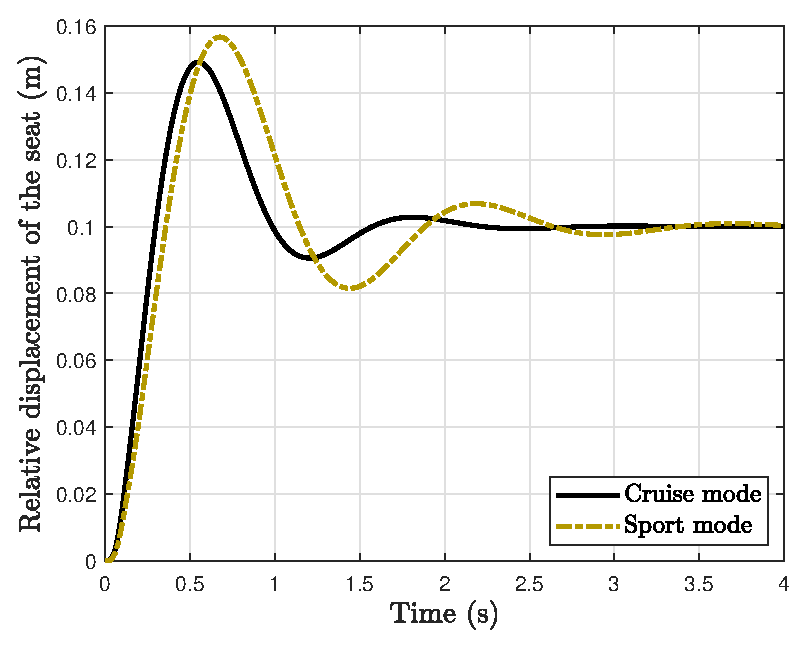
\includegraphics[width=0.9\textwidth]{./task1_seat.eps}
         \caption{Figure saved in the \texttt{.eps} file format.}
         \label{fig:three sin x}
     \end{subfigure}
        \caption{Three versions of the same figure for Task 1 of the assignment. Figure (a) is saved as ``\texttt{.jpg}'' and is fuzzy since this is not a vector format and the image has been rescaled. Figure (b) was obtained by taking a screenshot and cropping the image using \texttt{Microsoft Paint}. Again, the image is fuzzy and unclear. However, Figure (c) has been saved as a ``\texttt{.eps}''  which is a vector format which means that the clarity of the image is not lost as the image is rescaled. Getting clear images like this is an easy to make your report seem more professional and readable. }
        \label{fig:three graphs}
\end{figure}
\newpage
\bibliography{bibliog}

\end{document}
